\begin{figure}
\centering
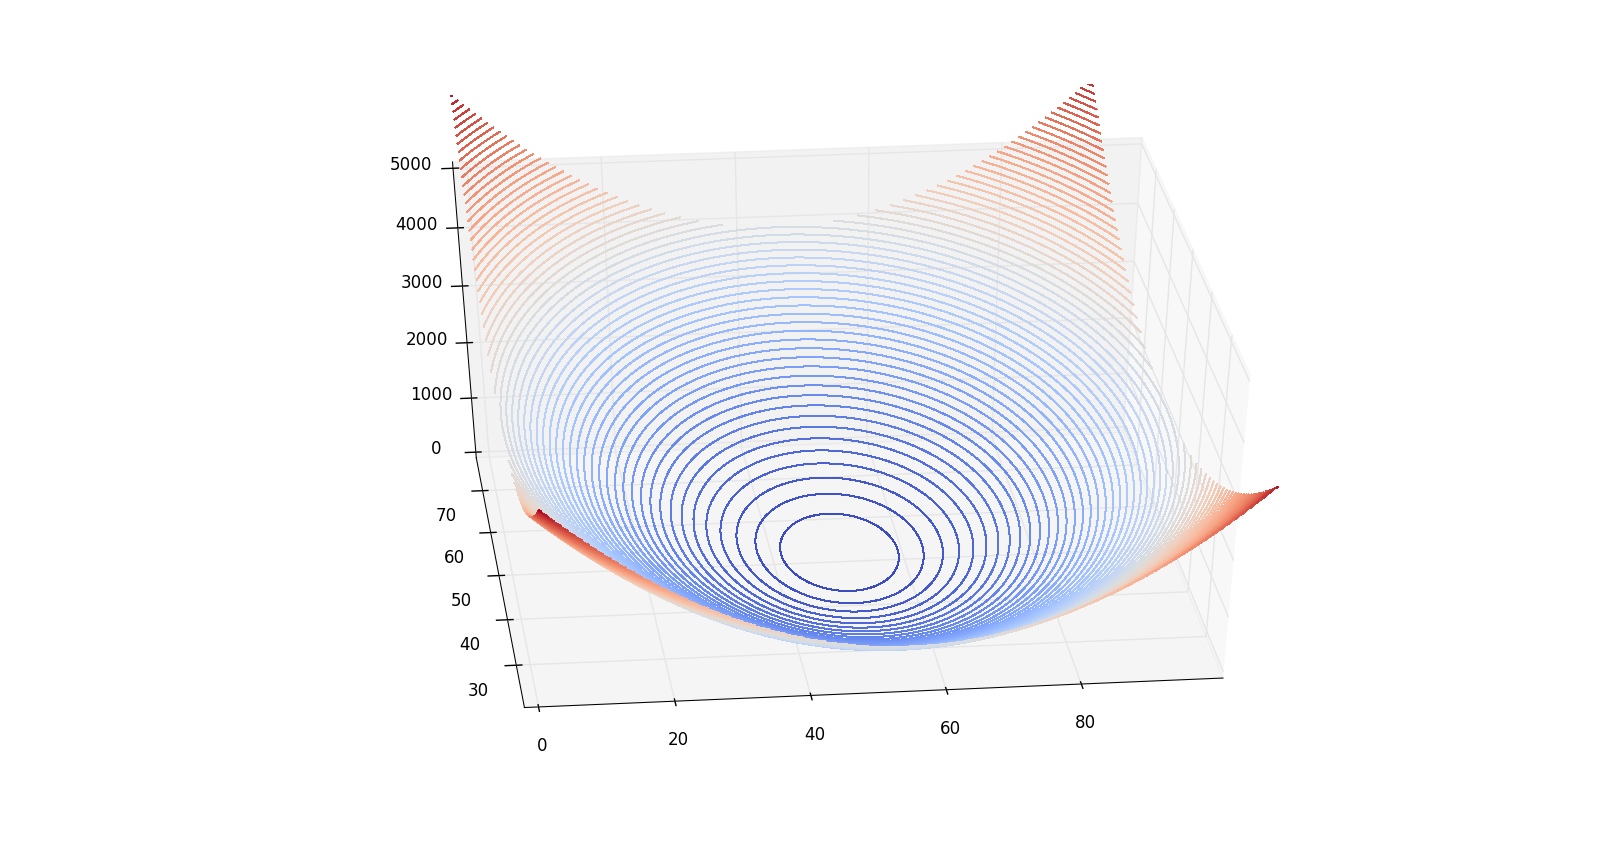
\includegraphics[height=.3\vsize]{fig/arriv1.png}
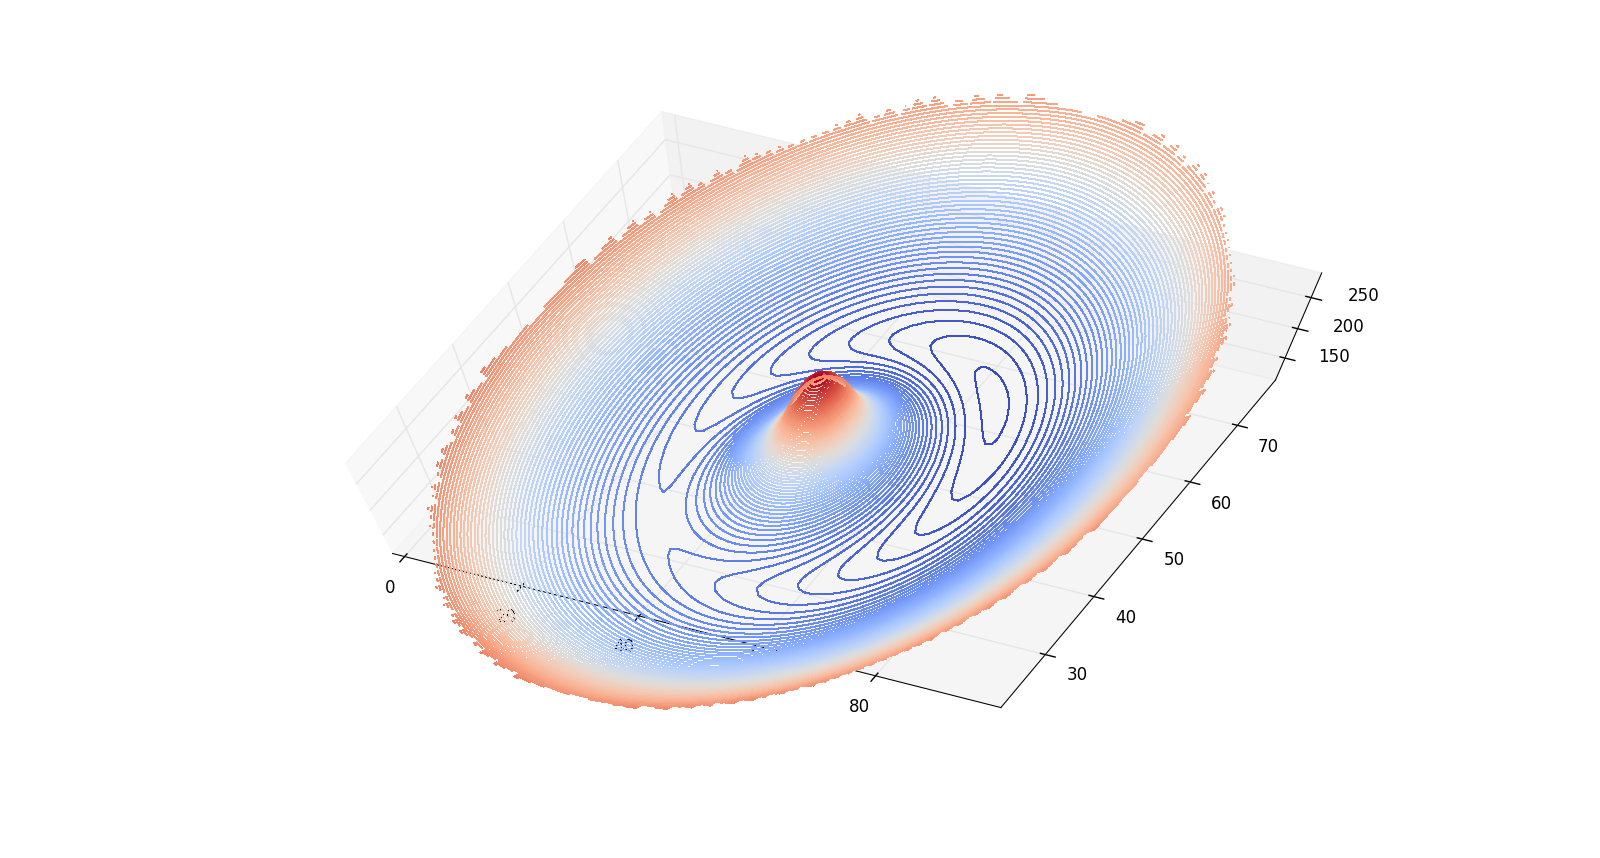
\includegraphics[height=.3\vsize]{fig/arriv2.png}
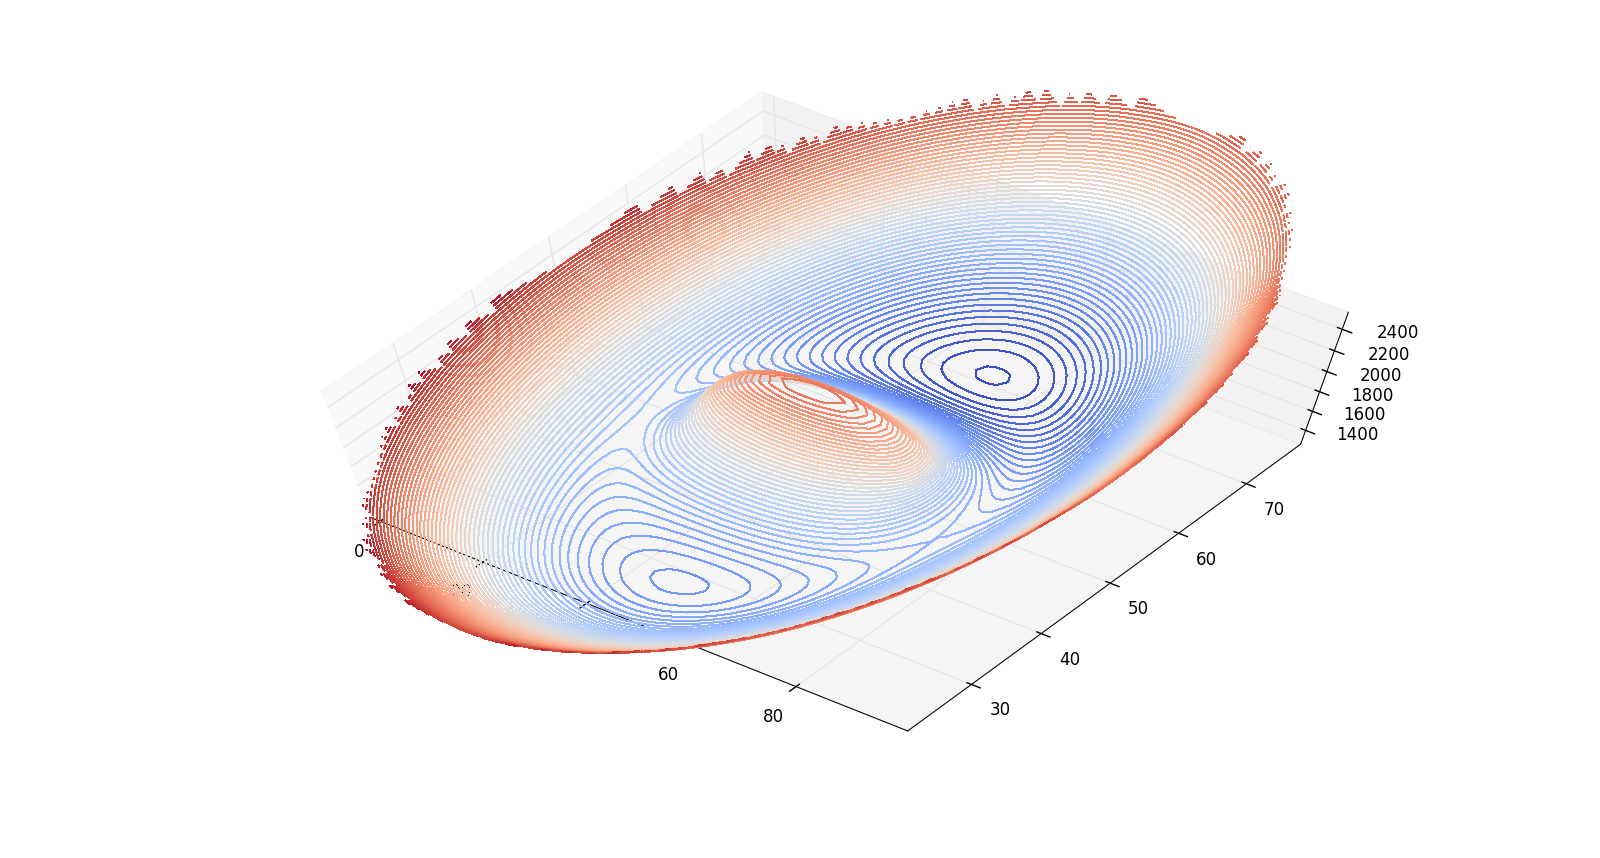
\includegraphics[height=.3\vsize]{fig/arriv3.png}
\caption{Arrival-time surfaces, with contour levels of equal arrival
  time.  The upper surface is with no lens.  The middle surface is
  when a circular lensing mass (offset from the source) is added; a
  maximum, a minimum and a saddle point can be seen.  The last surface
  is the result of an elongated lensing mass; a maximum, two minima
  and two saddle points can be seen.
}
\label{fig:arriv}
\end{figure}

\clearpage

\begin{figure}
  \centering
  \subfigure{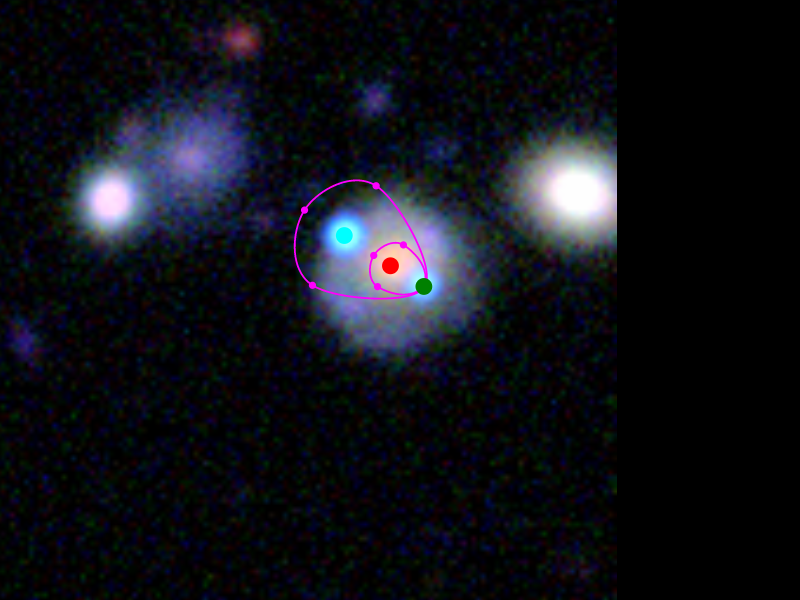
\includegraphics[width=0.45\textwidth]
             {fig/006941_input.png}} \\
  \subfigure{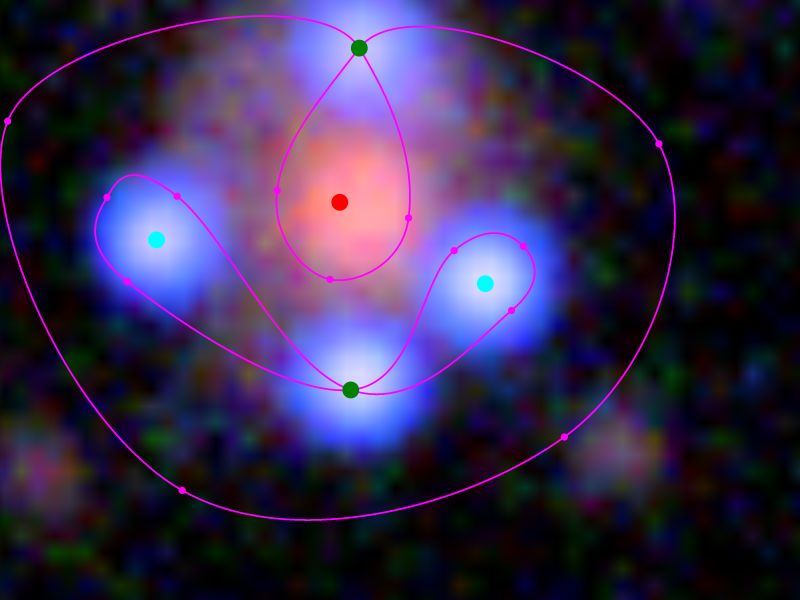
\includegraphics[width=0.45\textwidth]
             {fig/007022_input.png}} \\
  \subfigure{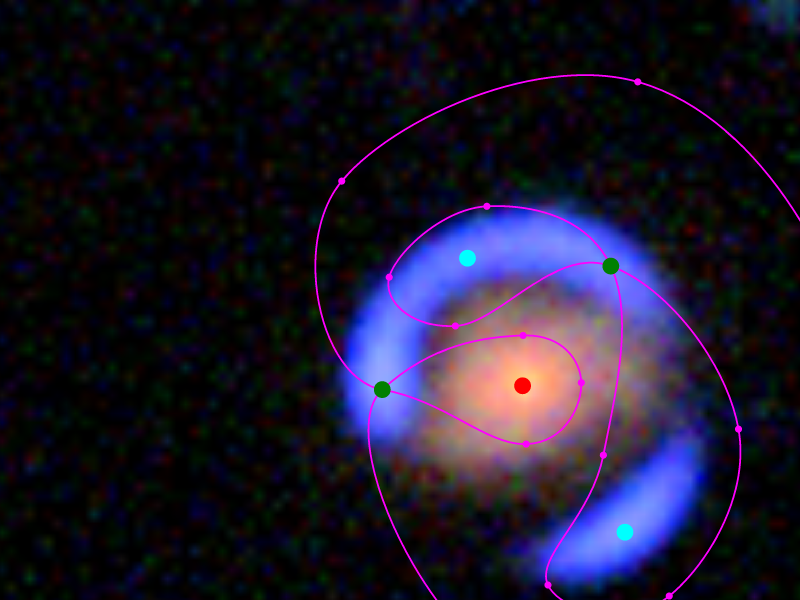
\includegraphics[width=0.45\textwidth]
             {fig/006919_input.png}}
  \caption{Examples of Spaghetti input.  The models from these appear
    later in Figures \ref{fig:6941}, \ref{fig:7022} and \ref{fig:6919}.
  }
  \label{fig:input-spag}
\end{figure}

\clearpage

\begin{figure}
  \centering
  \subfigure[real mass distribution]{
    \label{fig:6941_sim_mass}
    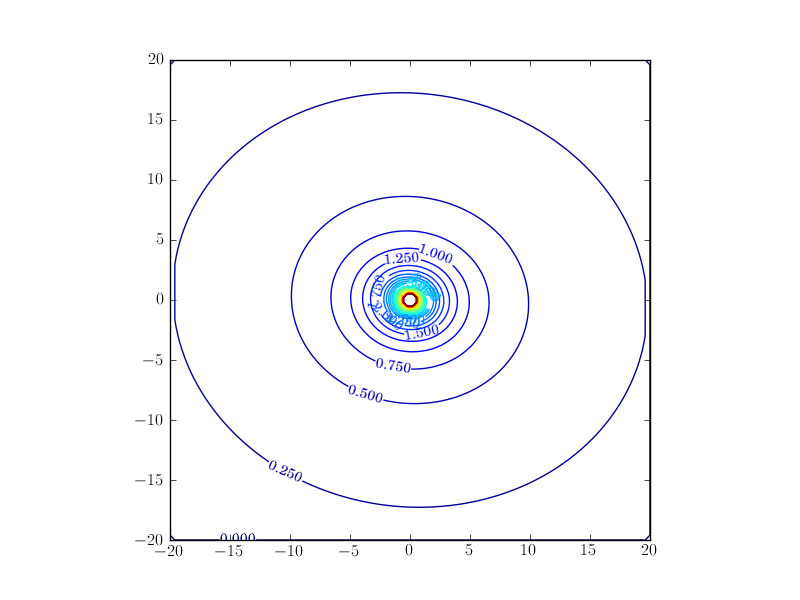
\includegraphics[width=0.45\textwidth]{fig/ASW000102p_kappa.png}
  }
  \subfigure[real arrival-time surface]{
    \label{fig:6941_sim_arr}
    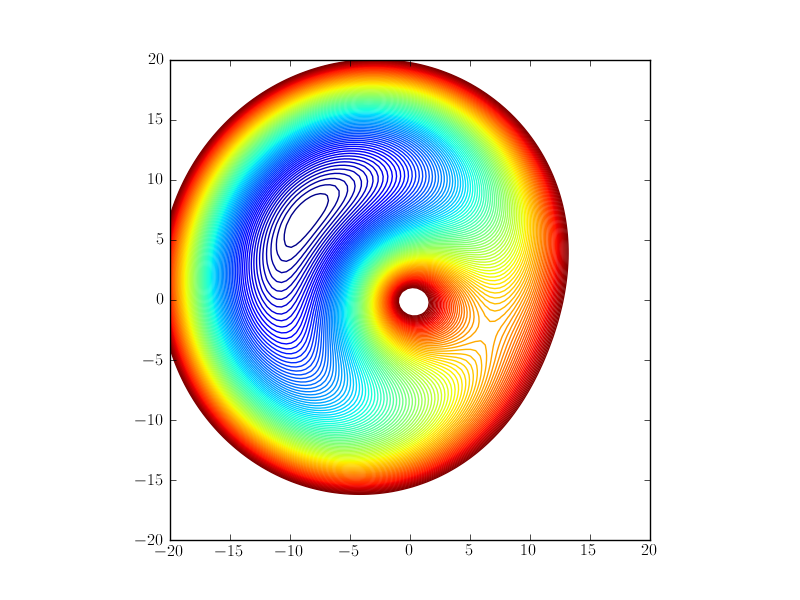
\includegraphics[width=0.45\textwidth]{fig/ASW000102p_arriv.png}
  }
  \subfigure[model mass distribution]{
    \label{fig:6941_mass}
    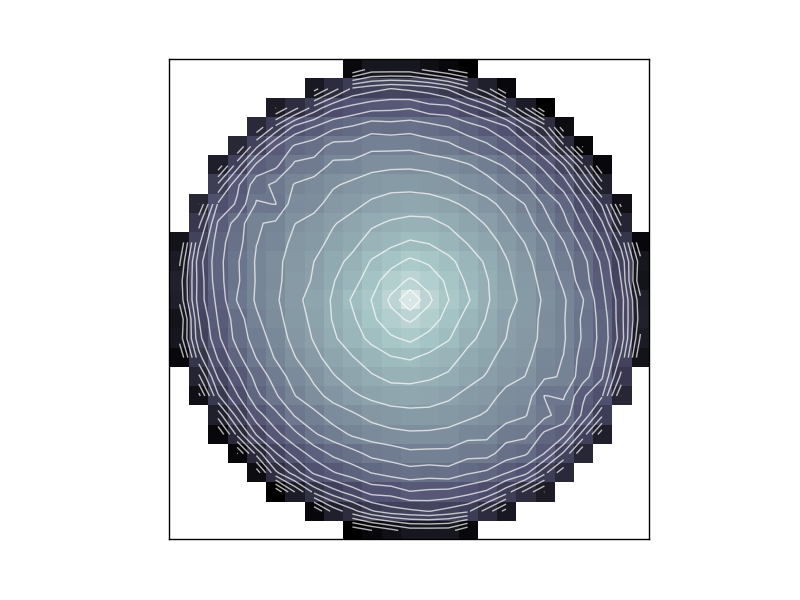
\includegraphics[width=0.45\textwidth]{fig/006941_mass.png}
  }
  \subfigure[model arrival-time surface]{
    \label{fig:6941_cont}
    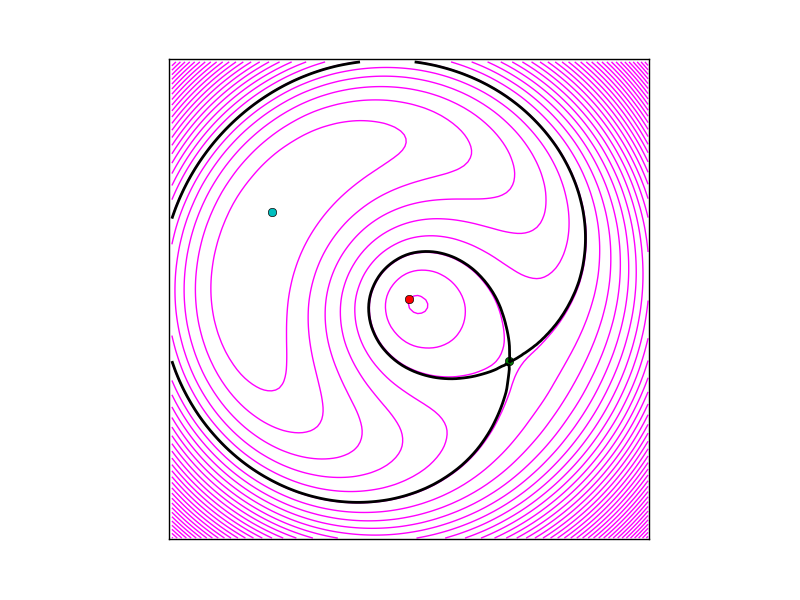
\includegraphics[width=0.45\textwidth]{fig/006941_spaghetti.png}
  }
  \subfigure[real vs model enclosed mass]{
    \label{fig:6941_kappa}
    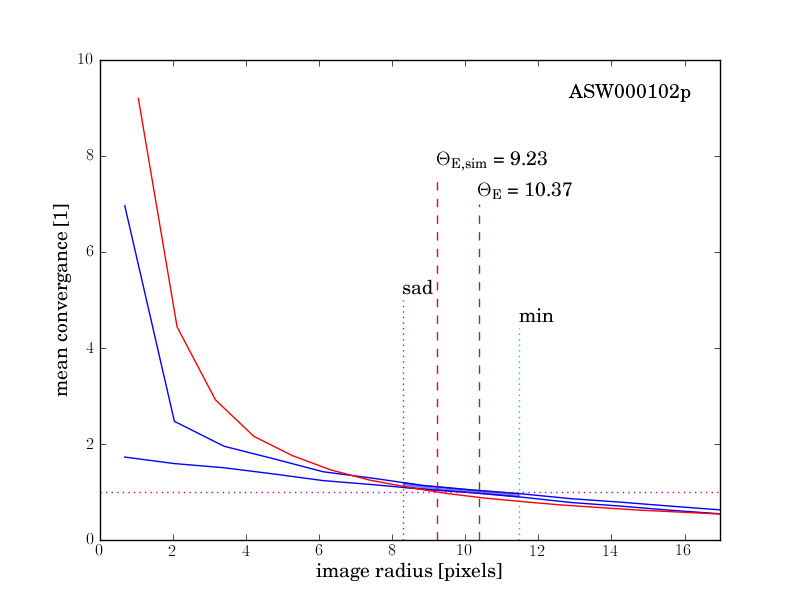
\includegraphics[width=0.45\textwidth]{fig/006941_kappa_encl.png}
  }
  \subfigure[model lensed image]{
    \label{fig:6941_atime}
    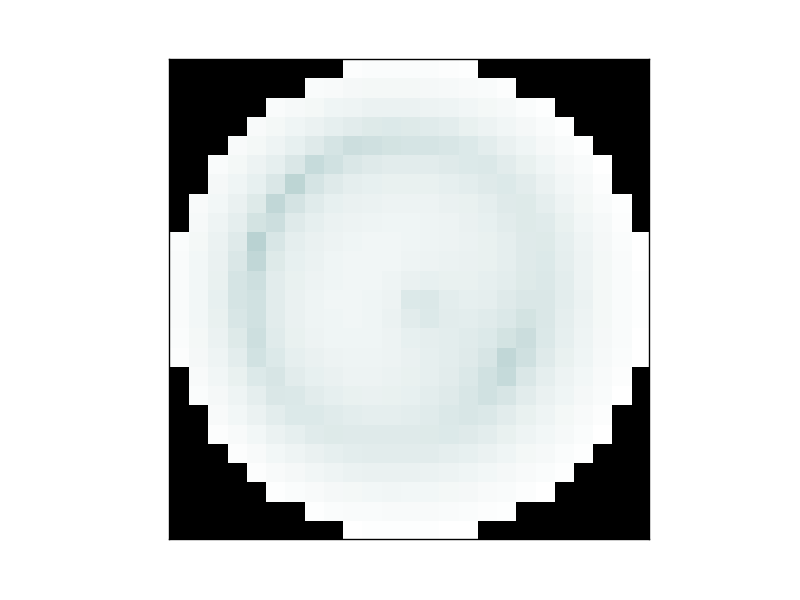
\includegraphics[width=0.45\textwidth]{fig/006941_arr_time.png}
  }

  \caption[result 6941 (ASW000102p)]{Sim ASW000102p and a model. Simple.}
  \label{fig:6941}
\end{figure}
  
\begin{figure}
  \centering
  \subfigure[real mass distribution]{
    \label{fig:6975_sim_mass}
    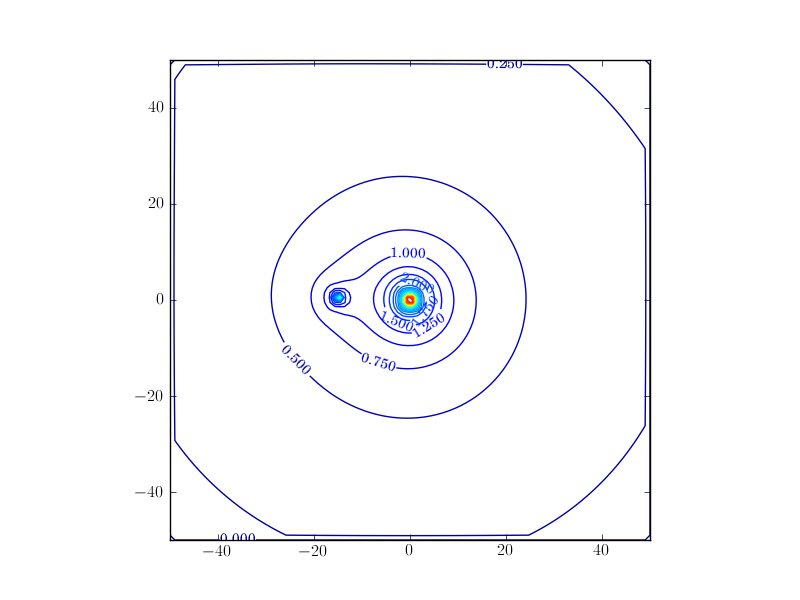
\includegraphics[width=0.45\textwidth]{fig/ASW000195x_kappa.png}
  }
  \subfigure[real arrival-time surface]{
    \label{fig:6975_sim_arr}
    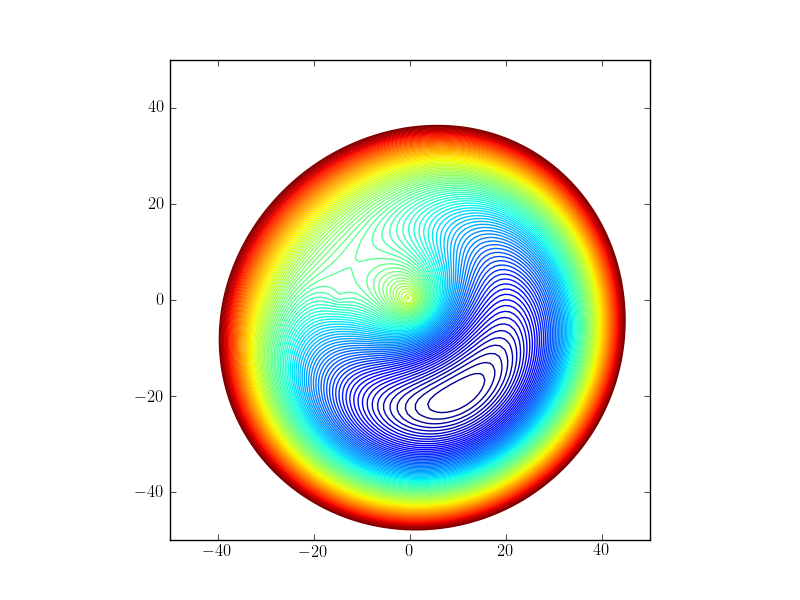
\includegraphics[width=0.45\textwidth]{fig/ASW000195x_arriv.png}
  }
  \subfigure[model mass distribution]{
    \label{fig:6975_mass}
    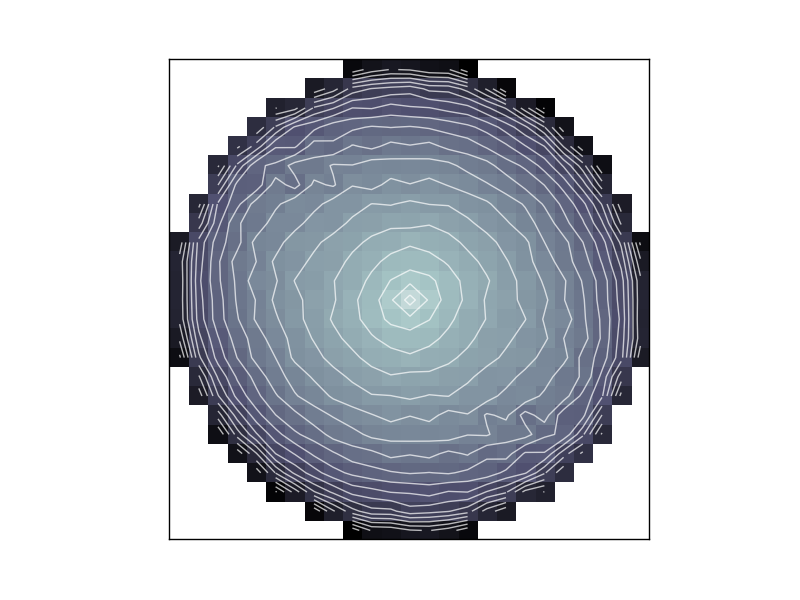
\includegraphics[width=0.45\textwidth]{fig/006975_mass.png}
  }
  \subfigure[model arrival-time surface]{
    \label{fig:6975_cont}
    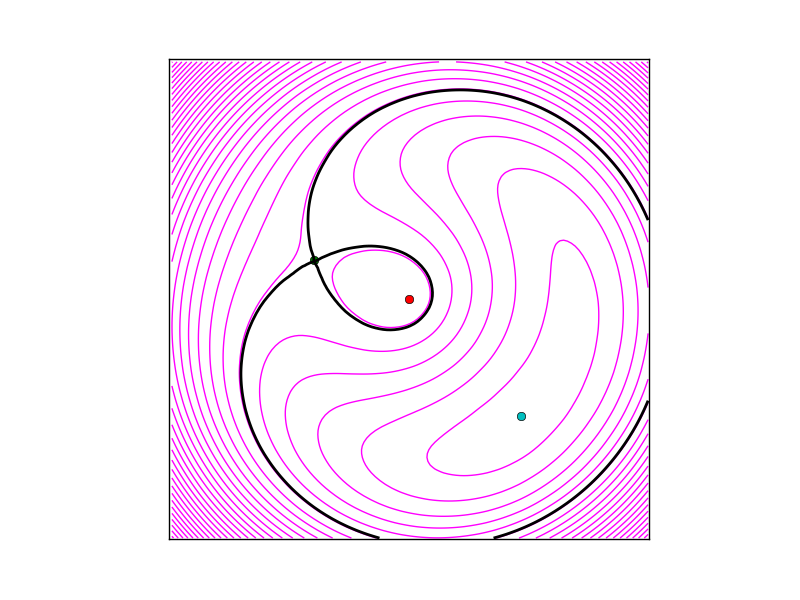
\includegraphics[width=0.45\textwidth]{fig/006975_spaghetti.png}
  }
  \subfigure[real vs model enclosed mass]{
    \label{fig:6975_kappa}
    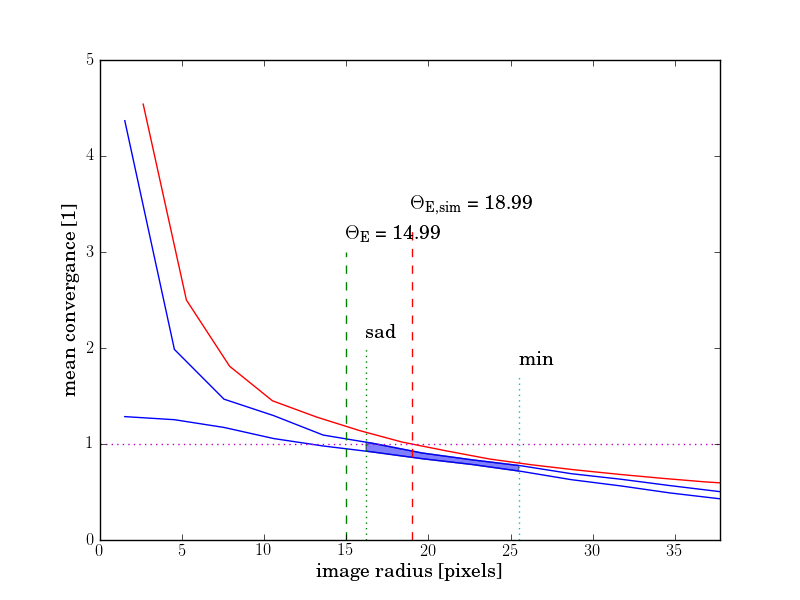
\includegraphics[width=0.45\textwidth]{fig/006975_kappa_encl.png}
  }
  \subfigure[model lensed image]{
    \label{fig:6975_atime}
    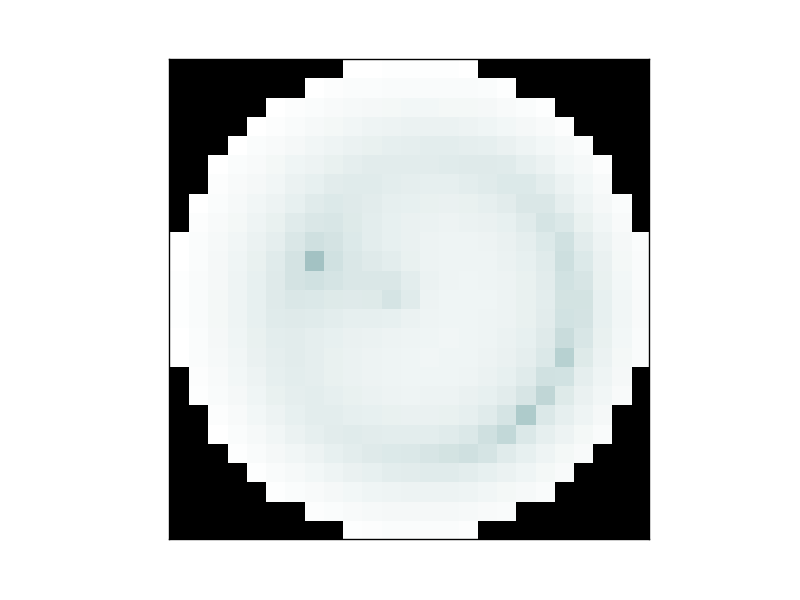
\includegraphics[width=0.45\textwidth]{fig/006975_arr_time.png}
  }

  \caption[result 6975 (ASW000195x)]{Sim ASW000195x and a model. Substructure ok.}
  \label{fig:6975}
\end{figure}
  
\begin{figure}
  \centering
  \subfigure[real mass distribution]{
    \label{fig:6937_sim_mass}
    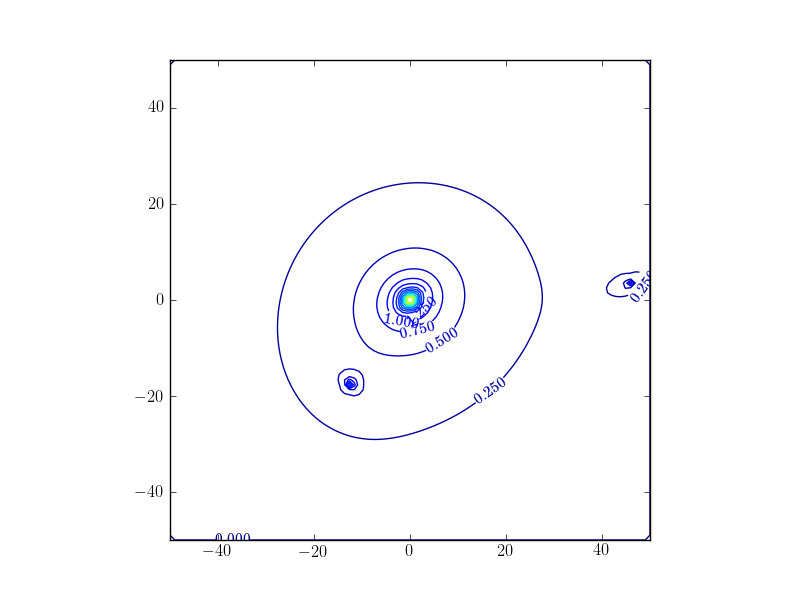
\includegraphics[width=0.45\textwidth]{fig/ASW0000vqg_kappa.png}
  }
  \subfigure[real arrival-time surface]{
    \label{fig:6937_sim_arr}
    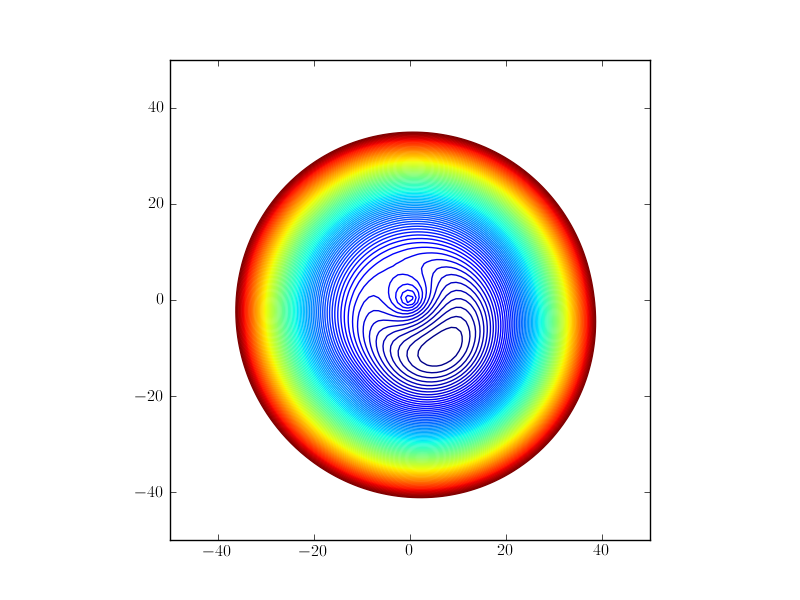
\includegraphics[width=0.45\textwidth]{fig/ASW0000vqg_arriv.png}
  }
  \subfigure[model mass distribution]{
    \label{fig:6937_mass}
    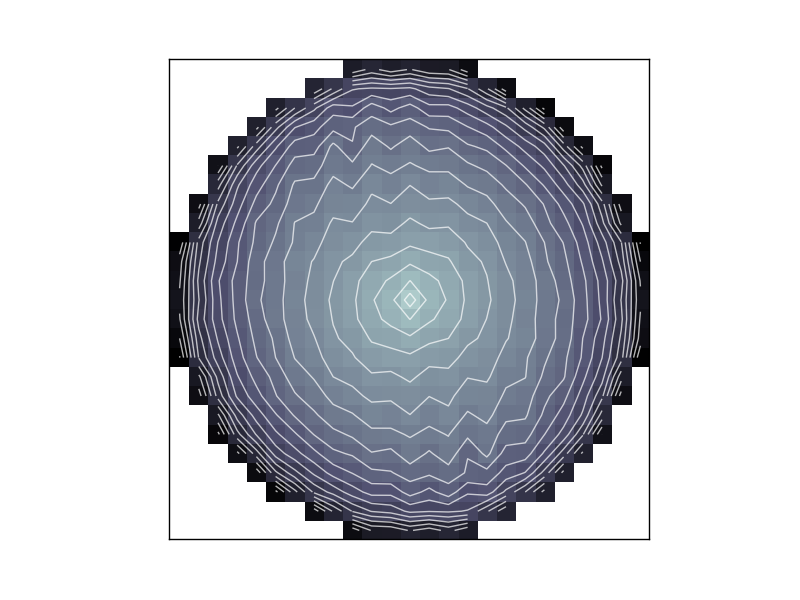
\includegraphics[width=0.45\textwidth]{fig/006937_mass.png}
  }
  \subfigure[model arrival-time surface]{
    \label{fig:6937_cont}
    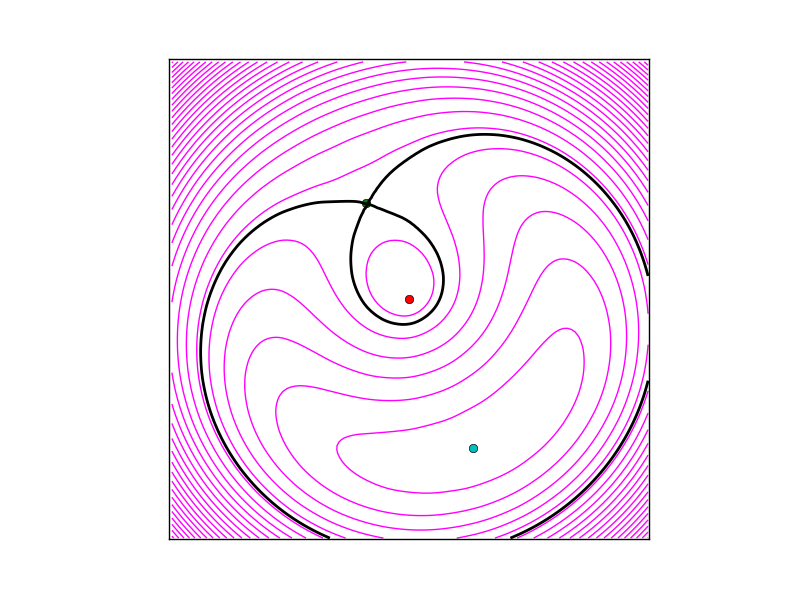
\includegraphics[width=0.45\textwidth]{fig/006937_spaghetti.png}
  }
  \subfigure[real vs model enclosed mass]{
    \label{fig:6937_kappa}
    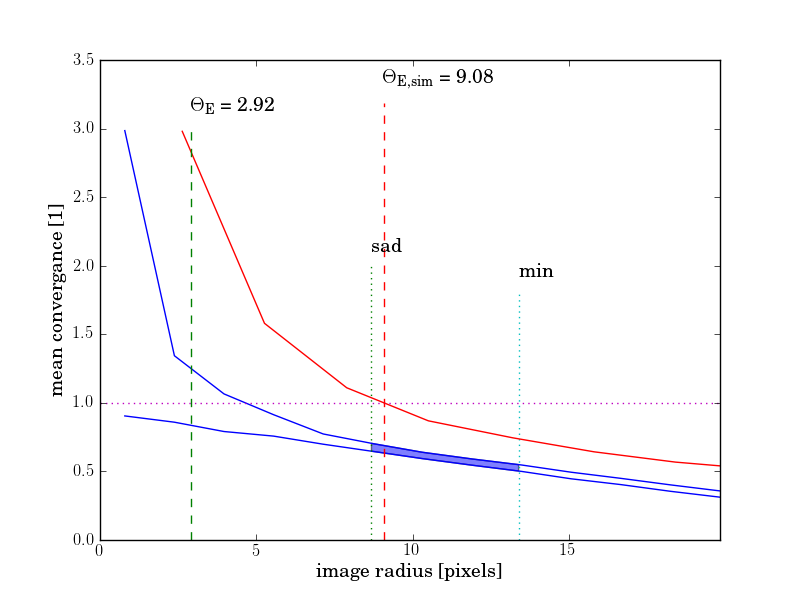
\includegraphics[width=0.45\textwidth]{fig/006937_kappa_encl.png}
  }
  \subfigure[model lensed image]{
    \label{fig:6937_atime}
    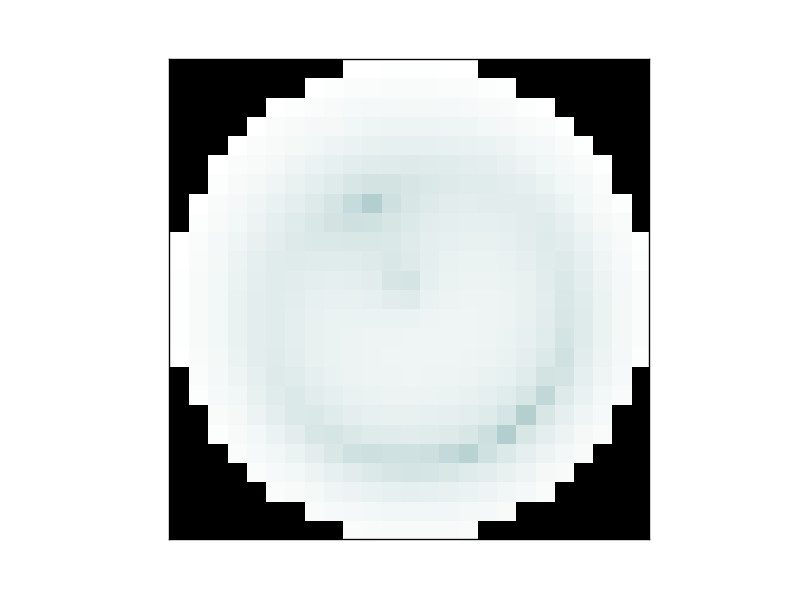
\includegraphics[width=0.45\textwidth]{fig/006937_arr_time.png}
  }

  \caption[result 6937 (ASW0000vqg)]{Sim ASW0000vqg and a model. Substructure fail.}
  \label{fig:6937}
\end{figure}
  
\begin{figure}
  \centering
  \subfigure[real mass distribution]{
    \label{fig:7022_sim_mass}
    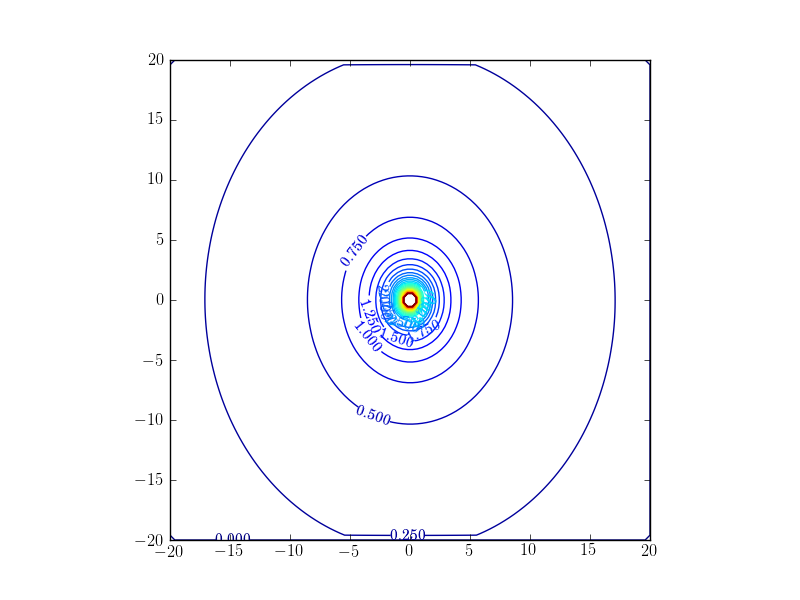
\includegraphics[width=0.45\textwidth]{fig/ASW0000h2m_kappa.png}
  }
  \subfigure[real arrival-time surface]{
    \label{fig:7022_sim_arr}
    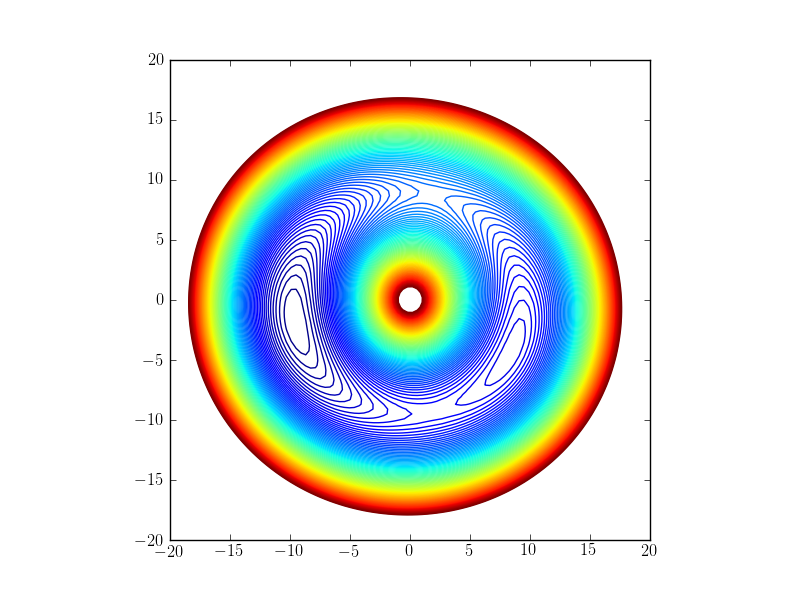
\includegraphics[width=0.45\textwidth]{fig/ASW0000h2m_arriv.png}
  }
  \subfigure[model mass distribution]{
    \label{fig:7022_mass}
    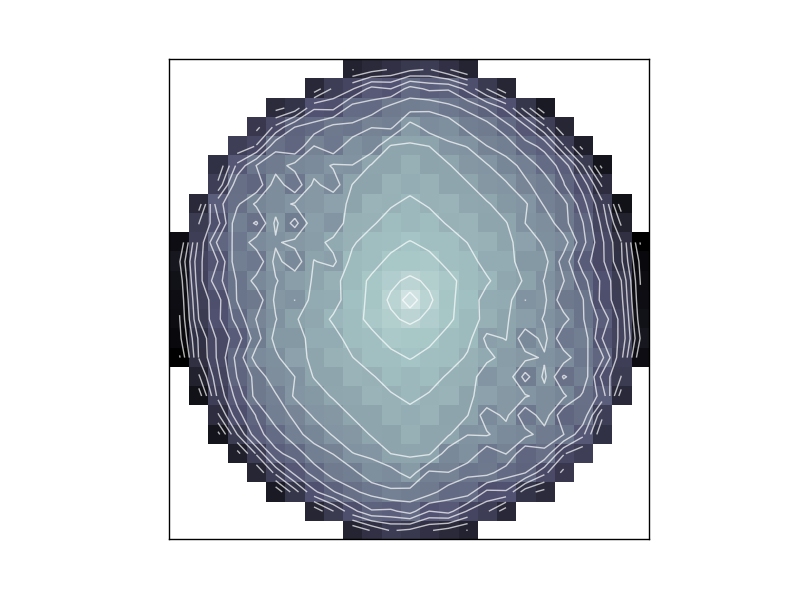
\includegraphics[width=0.45\textwidth]{fig/007022_mass.png}
  }
  \subfigure[model arrival-time surface]{
    \label{fig:7022_cont}
    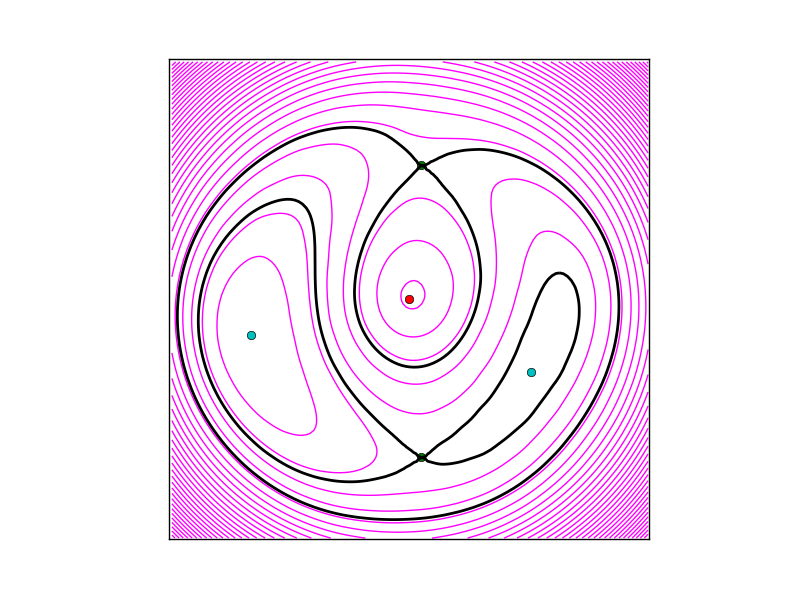
\includegraphics[width=0.45\textwidth]{fig/007022_spaghetti.png}
  }
  \subfigure[real vs model enclosed mass]{
    \label{fig:7022_kappa}
    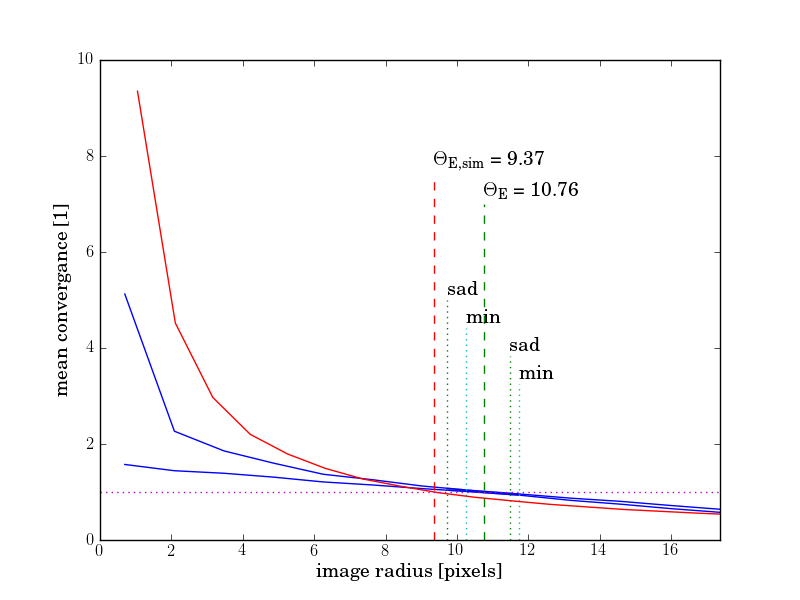
\includegraphics[width=0.45\textwidth]{fig/007022_kappa_encl.png}
  }
  \subfigure[model lensed image]{
    \label{fig:7022_atime}
    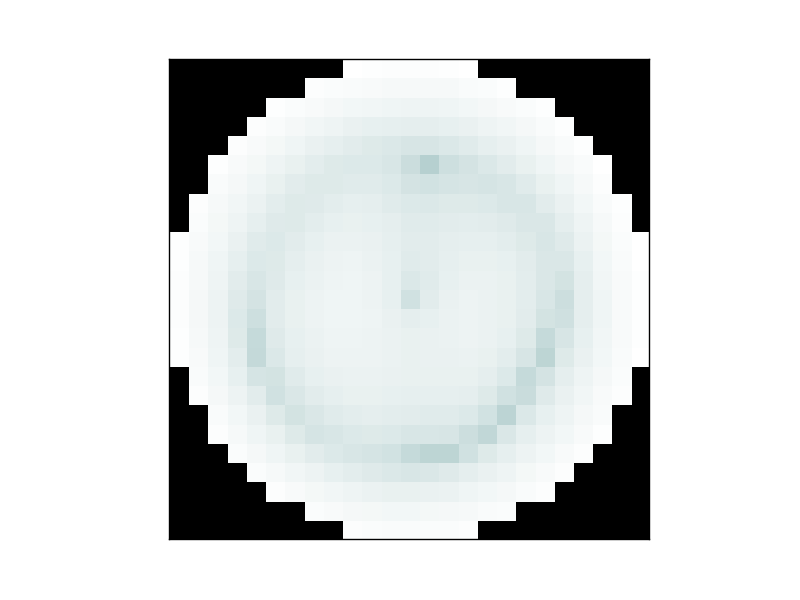
\includegraphics[width=0.45\textwidth]{fig/007022_arr_time.png}
  }

  \caption[result 7022 (ASW0000h2m)]{Sim ASW0000h2m and a model.  A core quad.}
  \label{fig:7022}
\end{figure}
  
\begin{figure}
  \centering
  \subfigure[real mass distribution]{
    \label{fig:7025_sim_mass}
    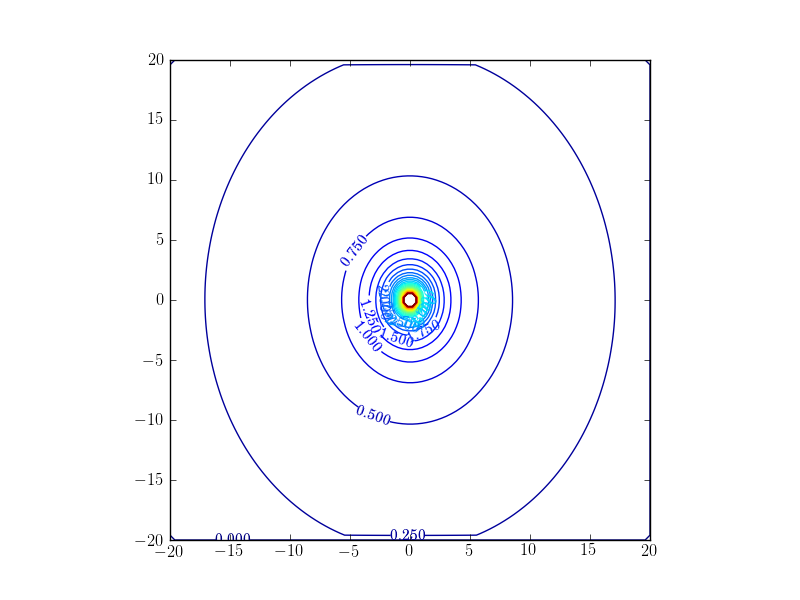
\includegraphics[width=0.45\textwidth]{fig/ASW0000h2m_kappa.png}
  }
  \subfigure[real arrival-time surface]{
    \label{fig:7025_sim_arr}
    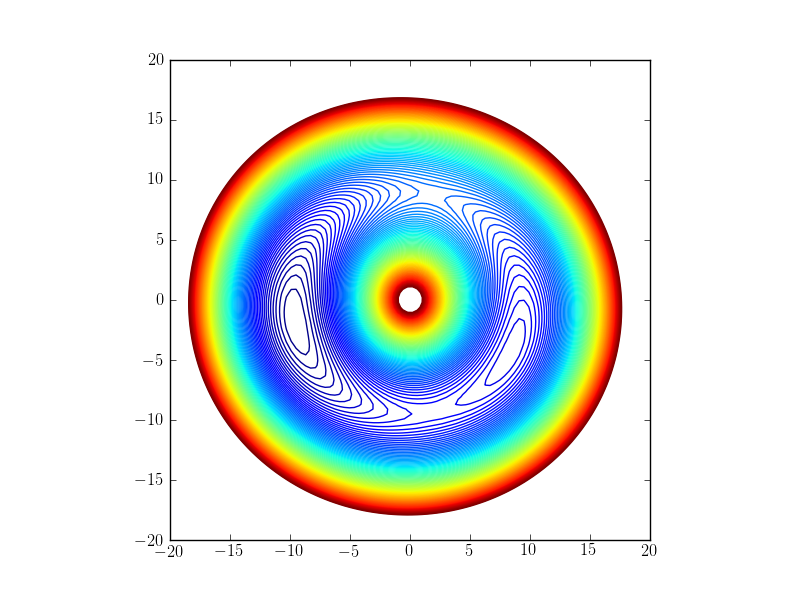
\includegraphics[width=0.45\textwidth]{fig/ASW0000h2m_arriv.png}
  }
  \subfigure[model mass distribution]{
    \label{fig:7025_mass}
    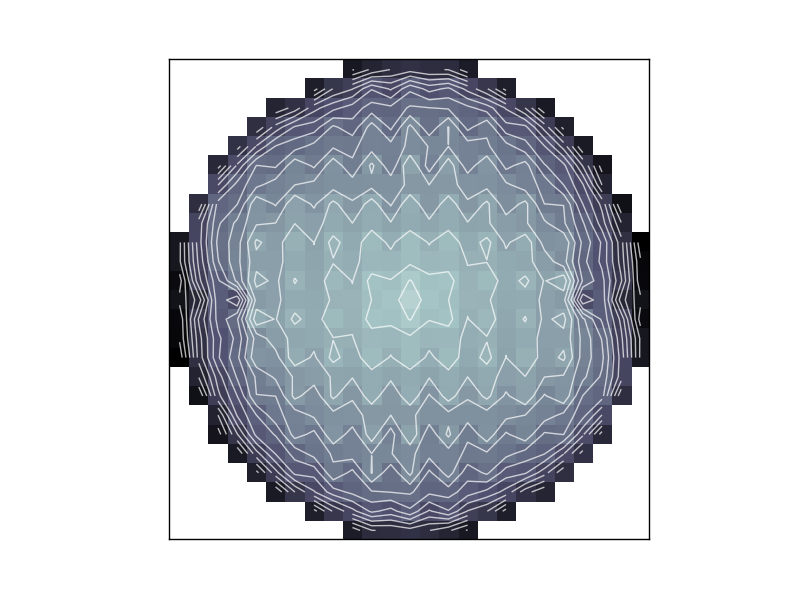
\includegraphics[width=0.45\textwidth]{fig/007025_mass.png}
  }
  \subfigure[model arrival-time surface]{
    \label{fig:7025_cont}
    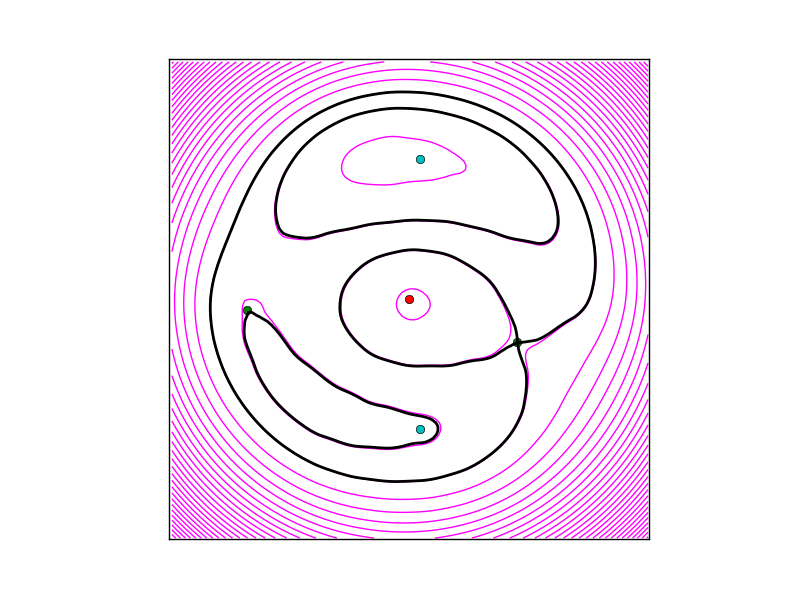
\includegraphics[width=0.45\textwidth]{fig/007025_spaghetti.png}
  }
  \subfigure[real vs model enclosed mass]{
    \label{fig:7025_kappa}
    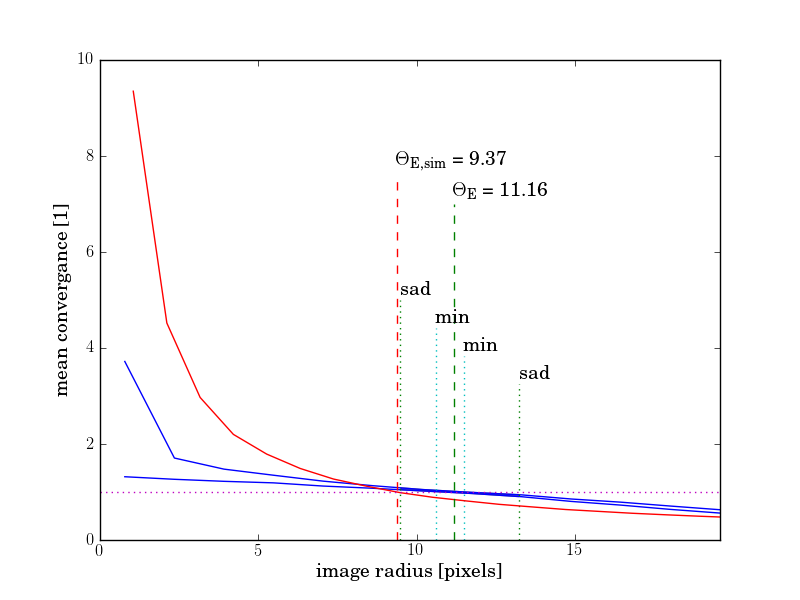
\includegraphics[width=0.45\textwidth]{fig/007025_kappa_encl.png}
  }
  \subfigure[model lensed image]{
    \label{fig:7025_atime}
    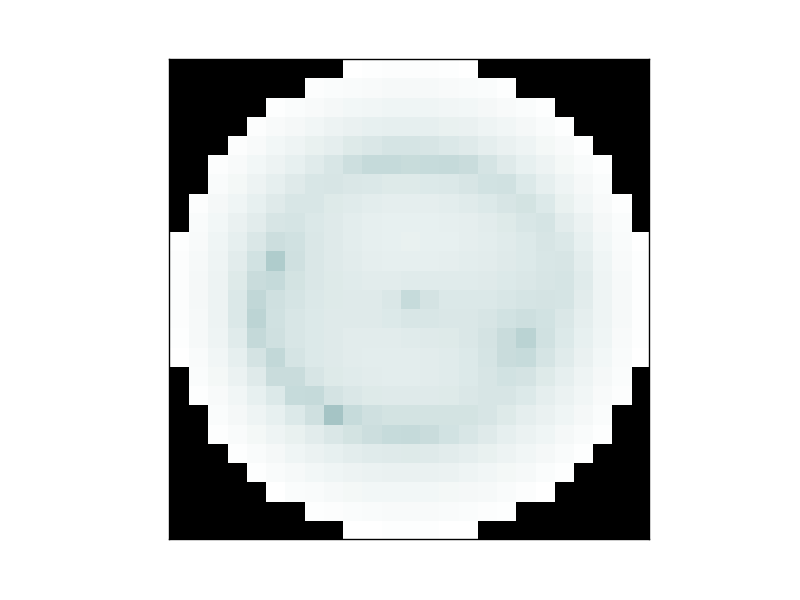
\includegraphics[width=0.45\textwidth]{fig/007025_arr_time.png}
  }

  \caption[result 7025 (ASW0000h2m)]{Sim ASW0000h2m and another model.  Wrong identification.}
  \label{fig:7025}
\end{figure}
  
\begin{figure}
  \centering
  \subfigure[real mass distribution]{
    \label{fig:6990_sim_mass}
    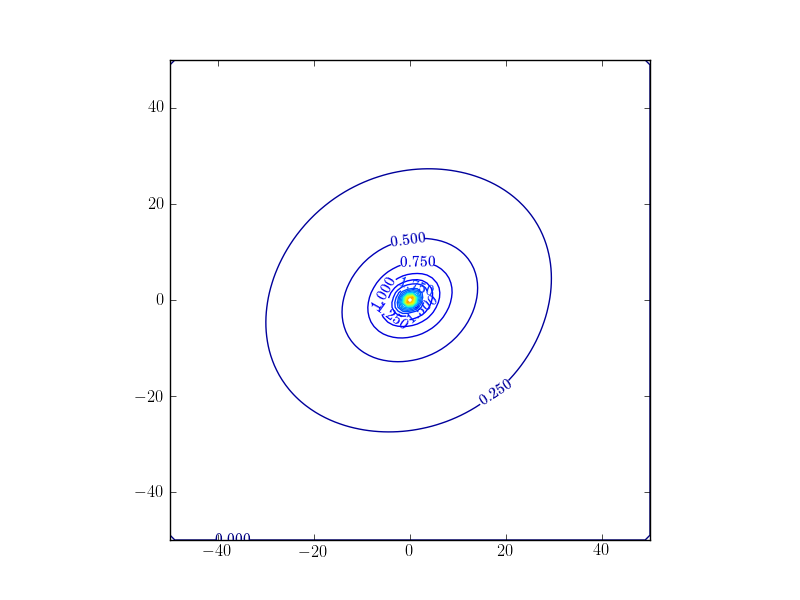
\includegraphics[width=0.45\textwidth]{fig/ASW0004oux_kappa.png}
  }
  \subfigure[real arrival-time surface]{
    \label{fig:6990_sim_arr}
    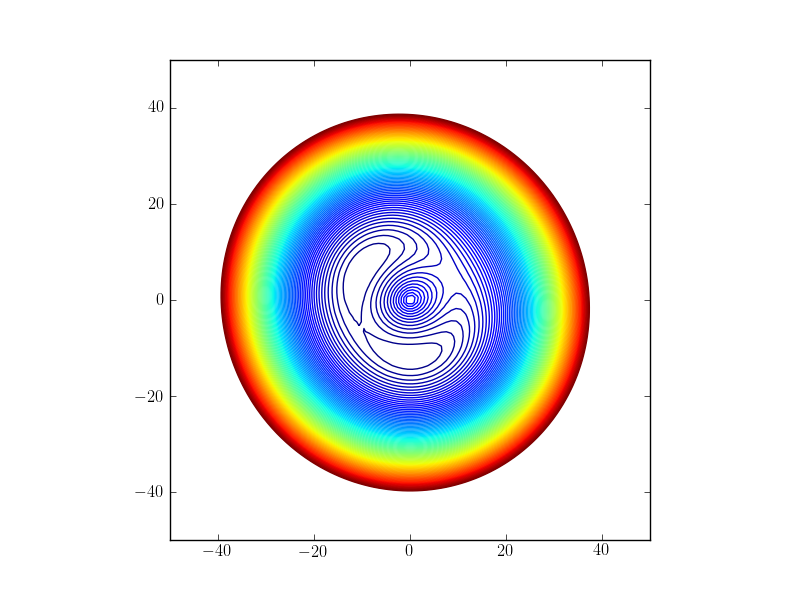
\includegraphics[width=0.45\textwidth]{fig/ASW0004oux_arriv.png}
  }
  \subfigure[model mass distribution]{
    \label{fig:6990_mass}
    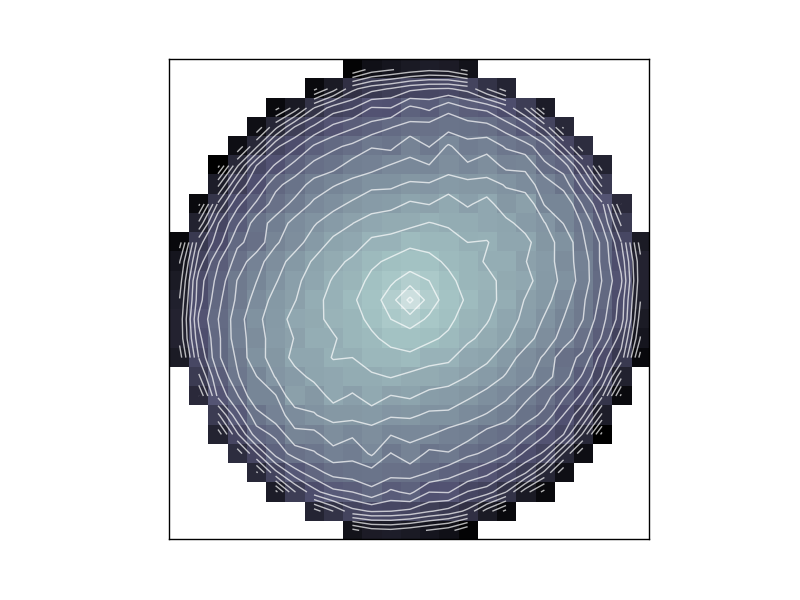
\includegraphics[width=0.45\textwidth]{fig/006990_mass.png}
  }
  \subfigure[model arrival-time surface]{
    \label{fig:6990_cont}
    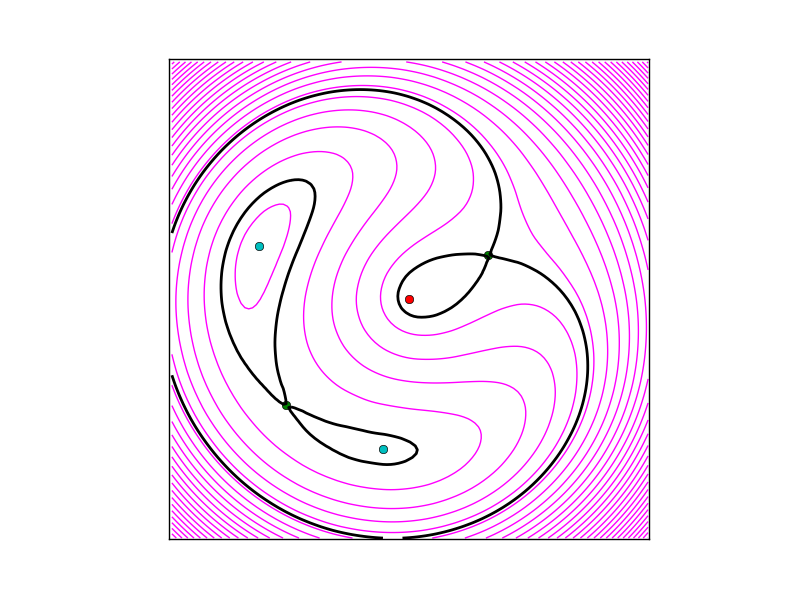
\includegraphics[width=0.45\textwidth]{fig/006990_spaghetti.png}
  }
  \subfigure[real vs model enclosed mass]{
    \label{fig:6990_kappa}
    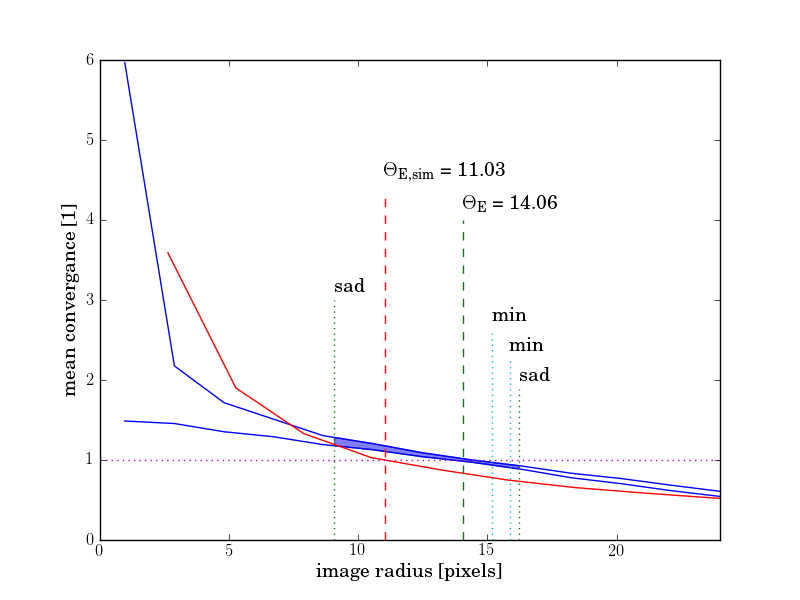
\includegraphics[width=0.45\textwidth]{fig/006990_kappa_encl.png}
  }
  \subfigure[model lensed image]{
    \label{fig:6990_atime}
    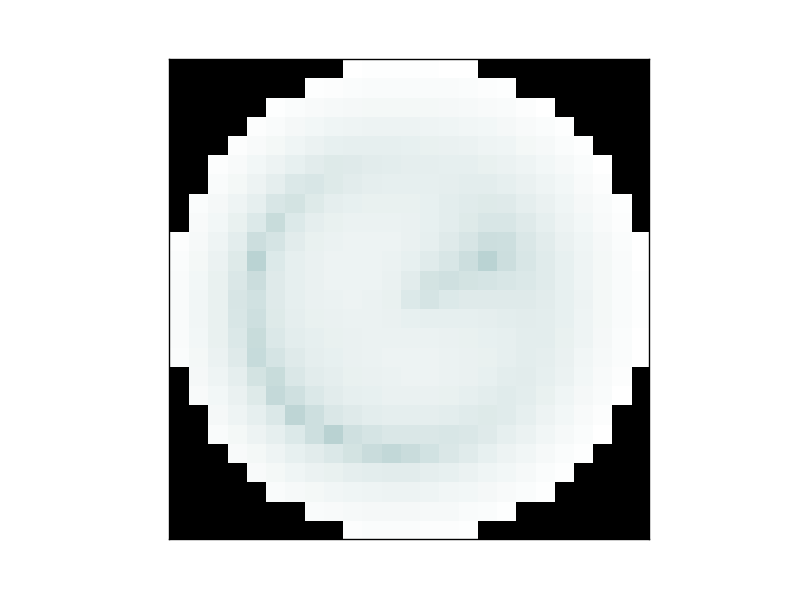
\includegraphics[width=0.45\textwidth]{fig/006990_arr_time.png}
  }

  \caption[result 6990 (ASW0004oux)]{Sim ASW0004oux and a model. A long-axis quad.}
  \label{fig:6990}
\end{figure}
  
\begin{figure}
  \centering
  \subfigure[real mass distribution]{
    \label{fig:6919_sim_mass}
    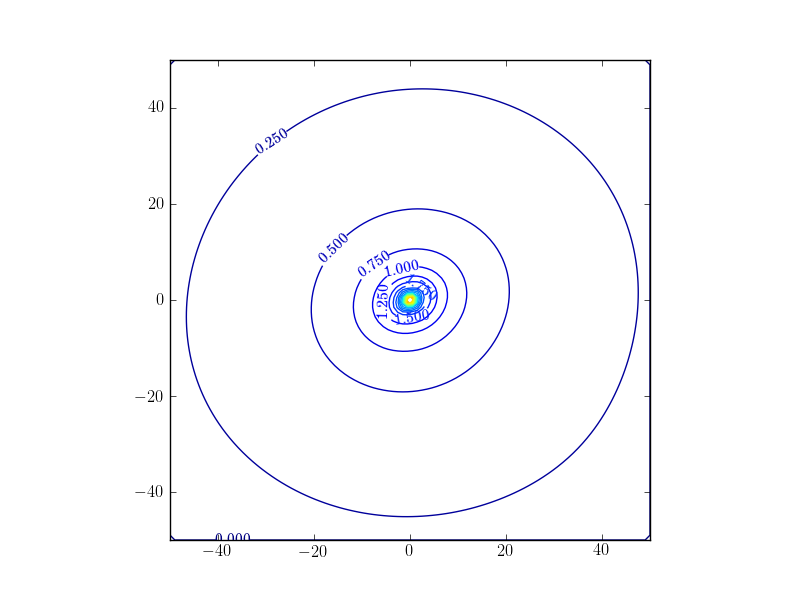
\includegraphics[width=0.45\textwidth]{fig/ASW0002z6f_kappa.png}
  }
  \subfigure[real arrival-time surface]{
    \label{fig:6919_sim_arr}
    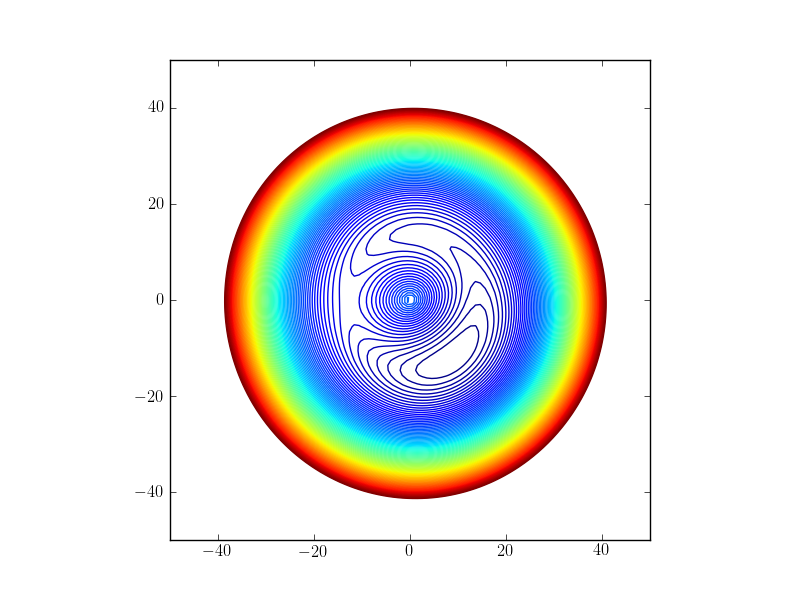
\includegraphics[width=0.45\textwidth]{fig/ASW0002z6f_arriv.png}
  }
  \subfigure[model mass distribution]{
    \label{fig:6919_mass}
    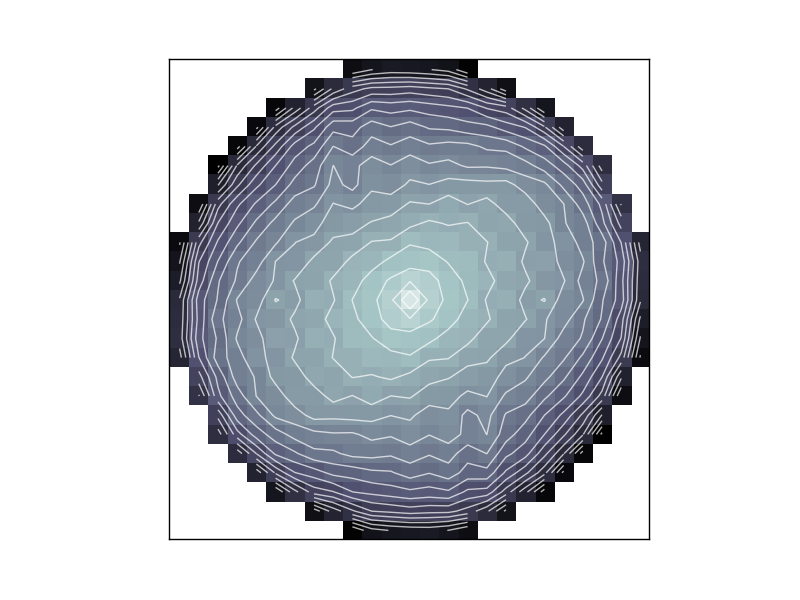
\includegraphics[width=0.45\textwidth]{fig/006919_mass.png}
  }
  \subfigure[model arrival-time surface]{
    \label{fig:6919_cont}
    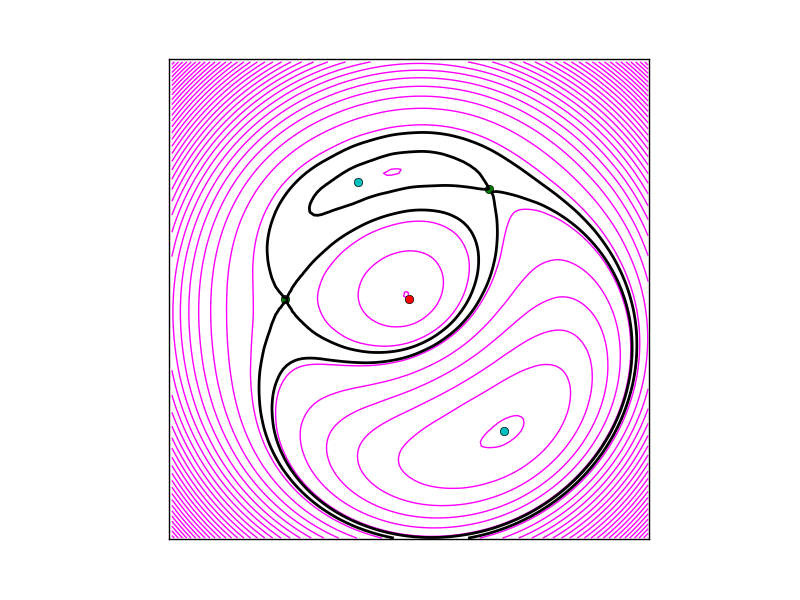
\includegraphics[width=0.45\textwidth]{fig/006919_spaghetti.png}
  }
  \subfigure[real vs model enclosed mass]{
    \label{fig:6919_kappa}
    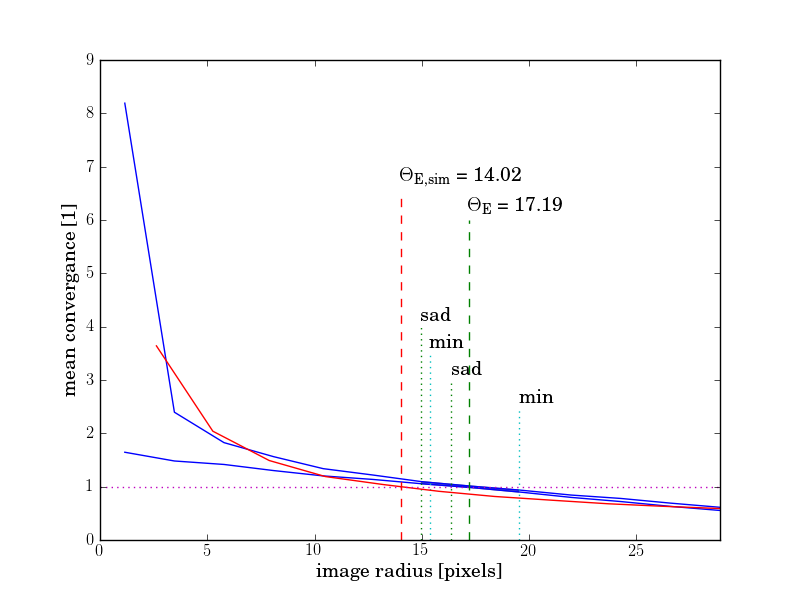
\includegraphics[width=0.45\textwidth]{fig/006919_kappa_encl.png}
  }
  \subfigure[model lensed image]{
    \label{fig:6919_atime}
    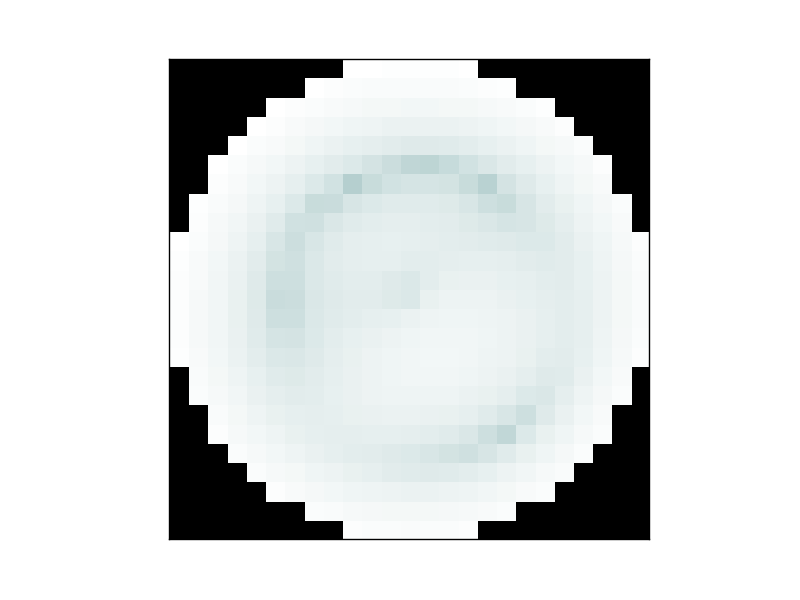
\includegraphics[width=0.45\textwidth]{fig/006919_arr_time.png}
  }

  \caption[result 6919 (ASW0002z6f)]{Sim ASW0002z6f and a model.  Incipient short-axis quad}
  \label{fig:6919}
\end{figure}
  
\begin{figure}
  \centering
  \subfigure[real mass distribution]{
    \label{fig:6915_sim_mass}
    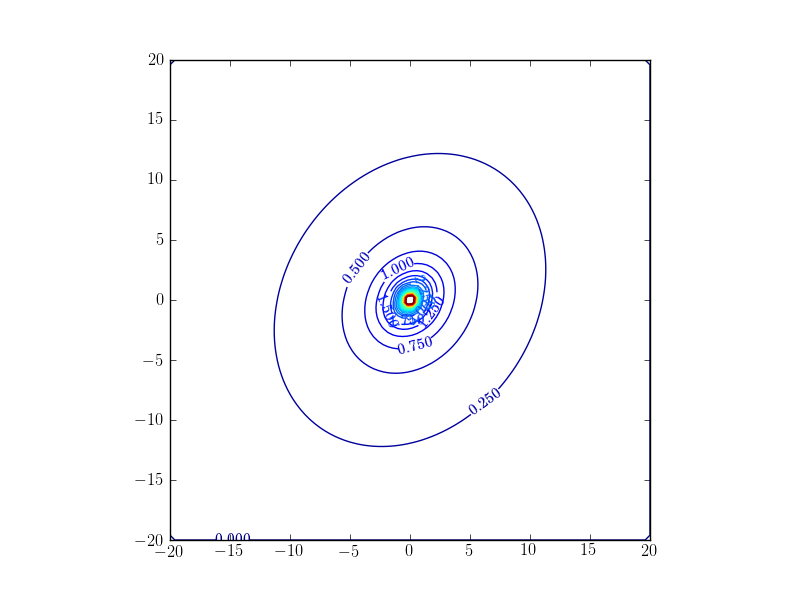
\includegraphics[width=0.45\textwidth]{fig/ASW0001hpf_kappa.png}
  }
  \subfigure[real arrival-time surface]{
    \label{fig:6915_sim_arr}
    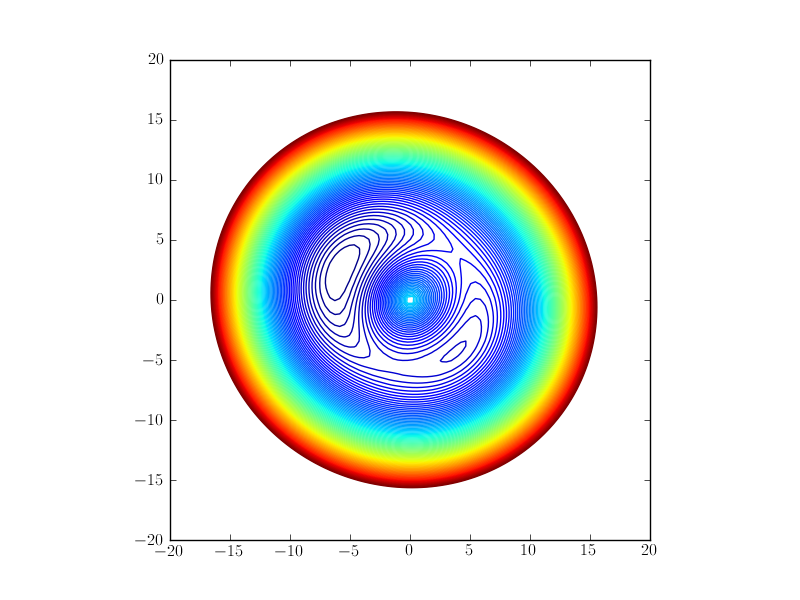
\includegraphics[width=0.45\textwidth]{fig/ASW0001hpf_arriv.png}
  }
  \subfigure[model mass distribution]{
    \label{fig:6915_mass}
    \includegraphics[width=0.45\textwidth]{fig/006915_mass.png}
  }
  \subfigure[model arrival-time surface]{
    \label{fig:6915_cont}
    \includegraphics[width=0.45\textwidth]{fig/006915_spaghetti.png}
  }
  \subfigure[real vs model enclosed mass]{
    \label{fig:6915_kappa}
    \includegraphics[width=0.45\textwidth]{fig/006915_kappa_encl.png}
  }
  \subfigure[model lensed image]{
    \label{fig:6915_atime}
    \includegraphics[width=0.45\textwidth]{fig/006915_arr_time.png}
  }

  \caption[result 6915 (ASW0001hpf)]{Sim ASW0001hpf and a model. Inclined quad.}
  \label{fig:6915}
\end{figure}

\clearpage

\begin{figure}[htbp]
  \centering
    \includegraphics[width=0.80\textwidth]{fig/eR_1.png}
  \caption{\ERf for all models with estimated errors in blue squares, \ERg of simulation in red crosses}
  \label{fig:ER_all_models}
\end{figure}

\begin{figure}[htbp]
  \centering
    \includegraphics[width=0.80\textwidth]{fig/eR_4.png}
  \caption{relative \ERf / \ERg[, sim] for models by volunteers (blue cross), models made by an expert (red cross with offset), including rejected models (green squares); binned per sim.}
  \label{fig:ER_per_sim}
\end{figure}

\begin{figure}
  \centering
  \subfigure{\includegraphics[width=0.45\textwidth]
             {fig/007020_kappa_encl}}
  \subfigure{\includegraphics[width=0.45\textwidth]
             {fig/007021_kappa_encl}} \\
  \subfigure{\includegraphics[width=0.45\textwidth]
             {fig/007024_kappa_encl}}
  \subfigure{\includegraphics[width=0.45\textwidth]
             {fig/007025_kappa_encl}}
  \subfigure{\includegraphics[width=0.45\textwidth]
             {fig/007022_kappa_encl}}
  \caption{\kenc for models of \asw{0h2m}: 7020 (top left), 7021 (top right), 7024 (mid left), 7025 (mid right) by volunteers and a correct model 7022 (bottom) by an expert.}
  \label{fig:kapenc_compare_faulty}
\end{figure}

